\documentclass[conference,letterpaper]{./../../IEEE/IEEEtran}

\usepackage{graphicx}
\usepackage{amsmath}
\usepackage{amsfonts}
\usepackage{algorithm}
\usepackage{algorithm,acronym}
\usepackage{subeqnarray,cite,mathtools,url}

\graphicspath{{./../Figures/}}
\DeclareGraphicsExtensions{.pdf}

\acrodef{MSE}{mean squared error}
\acrodef{IBC}{interference broadcast channel}
\acrodef{MC}{multi-cell}
\acrodef{BS}{base station}
\acrodef{MIMO}{multiple-input multiple-output}
\acrodef{SISO}{single-input single-output}
\acrodef{MU}{multiple users}
\acrodef{OFDM}{orthogonal frequency division multiplexing}
\acrodef{WSRM}{weighted sum rate maximization}
\acrodef{QoS}{quality of service}
\acrodef{SCA}{successive convex approximation}
\acrodef{SNR}{signal-to-noise ratio}
\acrodef{MMSE}{minimum \acl{MSE}}
\acrodef{SIR}{signal-to-interference ratio}
\acrodef{SINR}{signal-to-interference-plus-noise ratio}
\acrodef{Q-WSRM}{queue \acl{WSRM}}
\acrodef{QM}{queue minimizing}
\acrodef{SRA}{spatial resource allocation}
\acrodef{JSFRA}{joint space-frequency resource allocation}
\acrodef{WMMSE}{weighted \acl{MMSE}}
\acrodef{KKT}{Karush-Kuhn-Tucker}
\acrodef{GP}{geometric programming}
\acrodef{SOC}{second-order cone}
%\acrodef{BCDM}{block coordinate descent method}
\acrodef{ADMM}{alternating directions method of multipliers}
\acrodef{PD}{primal decomposition}
\acrodef{DD}{dual decomposition}
\acrodef{FFR}{fractional frequency reuse}
\acrodef{DC}{difference of convex}
\acrodef{Q-WSRME}{\ac{Q-WSRM} extended}
\acrodef{TDD}{time division duplexing}
\acrodef{CSI}{channel state information}
\acrodef{AO}{alternating optimization}
\acrodef{OTA}{over-the-air}
\acrodef{PL}{path loss}
\acrodef{TDM}{time division multiplexing}
\acrodef{UC}{uncoordinated}
\acrodef{SoC}{system-on-chip}
\acrodef{WMMSE}{weighted minimum mean squared error}
\acrodef{AMBA}{Advanced Microcontroller Bus Architecture}
\acrodef{AXI}{Advanced Extensible Interface}
\acrodef{FPGA}{Field-programmable gate array}
\acrodef{MSMCSRAM}{multi-core shared memory}
\acrodef{IPC}{inter-processor communications}
\acrodef{CIC}{chip-level interrupt controller}
\acrodef{MCSDK}{multi-core software development kit}
\acrodef{AMP}{Asymmetric Multi-Processing}
\newcommand{\mbf}[1]{\mathbf{#1}}
\newcommand{\me}[1]{\( #1 \)}
\newcommand{\mc}[1]{\mathcal{#1}}
\newcommand{\fall}{\forall}
\newcommand{\set}[1]{\left \lbrace #1 \right \rbrace }
\newcommand{\mvec}[2]{\mathbf{#1}_{#2}}
\newcommand{\ith}[1]{{#1}^\mathrm{th}}
\newcommand{\pr}[1]{{#1}^\prime}
\newcommand{\mbfa}[1]{{\boldsymbol{#1}}}
\newcommand{\herm}{\mathrm{H}}
\newcommand{\sset}[1]{\left [ #1 \right ]}
\newcommand{\rfrac}[2]{{}^{#1}/{}_{#2}}
\newcommand{\eqspace}{\IEEEeqnarraynumspace}
\newcommand{\enoise}{\widetilde{N}_0}
\newcommand{\eqsub}{\IEEEyessubnumber}
\newcommand{\review}[1]{{\textcolor[rgb]{0 0 0.6}{#1}}}
\newcommand{\trace}{\mathrm{tr}}
\newcommand{\tran}{\mathrm{T}}
\newcommand{\R}[1]{\label{#1}\linelabel{#1}}
\newcommand{\lr}[1]{page~\pageref{#1}, line~\lineref{#1}}
\newcommand{\eqn}[1]{\(#1\)}
\newcommand{\mx}{\mbf{m}}
\newcommand{\my}{\mbf{w}}
\newcommand{\mz}{\mbfa{\gamma}}
\newcommand{\mxb}{{{\mbf{m}}}}
\newcommand{\myb}{{{\mbf{w}}}}
\newcommand{\iterate}[2]{{#1}^{(#2)}}
\newcommand{\iter}[3]{{#1}_{#2}^{(#3)}}
\newcommand{\ma}{\mbf{x}}

\begin{document}

\title{Exploiting Multi-Core SoC Architecture for MU-MIMO Schedulers}
%\vspace{-22ex}

\author{\begin{tabular}{cc}
\multicolumn{2}{c}{Ganesh Venkatraman, Janne Janhunen, Markku Juntti}\\
Centre for Wireless Communications (CWC), & Department of Communication Engineering (DCE), \\
\multicolumn{2}{c}{FI-90014, University of Oulu, Finland}\\
\end{tabular}}

\maketitle

\begin{abstract}
Upcoming standards are moving towards multi-antenna multiple-input multiple-output (MIMO) transmission techniques to harness the benefits of spatial degrees of freedom (DoF) in addition to the conventional time and frequency resources. Even though single user MIMO transmission improves the throughput noticeably, multiplexing different user data streams across the spatial dimension as in multi-user (MU) MIMO enhances the overall cell throughput significantly. However, this improved performance depends on the efficient selection of the users to be multiplexed over the spatial DoF. In this work, we compare the performance of different scheduling schemes in terms of achievable sum throughput and the overall complexity involved in the implementation for the real-time system requirements. The performances of the proposed schemes are evaluated on MATLAB for various MIMO configurations. The complexity analysis is carried out by implementing the scheduler algorithms on TI TCI6636K2H evaluation platform. We evaluate the complexity by sharing the load across eight TMS320C66x DSP core subsystem on the (system-on-chip) SoC.
\end{abstract}

\acused{MIMO}
\acresetall
\section{Introduction}
The current wireless standards are moving towards the packet switched networks to improve the system performance and flexibility as compared to the circuit switched networks. The radio access technologies aim at achieving higher throughput and better system performance but still targeting at low energy budget. The use of multi-antenna transmission is \textit{de-facto} in all upcoming wireless access standards, favoring the spatial multiplexing of user data by applying transmit precoders for multi-user \ac{MIMO} transmission. In order to achieve the best possible benefit of the multi-user (MU) \ac{MIMO} transmission, the multiplexed users should have channel vectors as linearly independent as possible. By selecting users with the uncorrelated channel vectors, efficient linear precoders can be designed to decouple the user data streams and to avail the benefits of MU-MIMO technique. The selection of users with such a constraint is carried out by the schedulers to utilize the wireless system resources efficiently.

The scheduling algorithms based on the sum rate maximization objective for MU-MIMO were discussed thoroughly in the literature. The search based on successive projections (SP) scheme for single-antenna receiver was presented in \cite{sus2006zfbf} and its extension to the multi-antenna receivers was provided in \cite{Tolli-etal-2005}. In \cite{Tolli-etal-2005}, the users were selected iteratively by choosing the channel vector with the maximum gain onto the orthogonal subspace. The orthogonal subspace was obtained by evaluating the null space of the stacked channel vectors of the already chosen users from the earlier iterations. Similar algorithms addressing a lower computational complexity were proposed in \cite{shen2006low} and \cite{youtuan2007improved}. User selection based on the volume maximization metric was discussed in \cite{jin2010novel}. It is identical to the SP or the block diagonal (BD) scheme, since both are based on Gram-Schmidt (GS) procedure to find the orthogonal vectors.

Even though the scheduling algorithm determines a subset of users from a large set of contending users, precoders are to be designed efficiently to harness wireless resources effectively. The iterative precoder design based on the \ac{MSE} reformulation for the \ac{WSRM} objective provides an efficient transmit precoder design \cite{wmmse_shi}. The precoders can be used to determine the subset of users implicitly by assigning all-zero vector as the precoder for the unscheduled users. However, the complexity involved in the precoder design scales significantly with the number of users for which the precoders are to be designed as compared to the elementary design based on zero-forcing (ZF) criterion. Even though the ZF based precoder design is inferior to the \ac{WMMSE} approach, it provides a closed form expression to evaluate the precoder design followed by a bisection search to identify the power for each data stream. The choice of precoder design also plays a major role in the achievable sum rate.

In this paper, we focus on the efficient implementation of various state-of-the-art MU-MIMO scheduling algorithms on a multi-core \ac{SoC} platform and evaluate the system size that can be supported with the current implementation. In order to have a fair comparison, we first analyze the achievable throughput by different algorithms and then we discuss the implementation complexity of the scheduling algorithms on TI TCI6636K2H evaluation platform. This work is a continuation to our previous implementation studies \cite{Janhunen-etal-11, Hanninen-etal-2014, Shahabuddin-etal-2014} aiming at finding low-power but high performance solutions for the advanced long term evolution (LTE-A) transceivers. Current work excludes the precoding design, but it is based on the two-step scheduling-precoding approach, where the scheduler finds a subset of users in the first and in the second step, the precoders are designed for the chosen subset.

The paper is organized as follows. A single-cell downlink system model is described in Section \ref{sec:system_model} followed by a brief discussion on the scheduler algorithms in Section \ref{sec:sched_discussions}. Section \ref{sec:perf_scheduling} compares the performance between selected scheduler schemes using link level simulations. In Section \ref{sec:implementation}, implementation results of different scheduling algorithms are presented. Section \ref{sec:conclusion} summarizes the conclusions.

\section{System Model}
\label{sec:system_model}
We consider a single-cell downlink MU-MIMO transmission with \eqn{N_T} transmit antennas and \eqn{K} users with \eqn{N_R} antenna each. Let \eqn{\mvec{H}{k} \in \mathbb{C}^{N_R \times N_T}} be the channel matrix seen by user \me{k}. Let \me{\kappa = \min(N_R,N_T)} be the rank of channel matrix \me{\mvec{H}{k}}. To utilize the available spatial streams, the channel matrix \eqn{\mvec{H}{k}} is decomposed into \me{N_R} virtual single receive antenna channel vectors using singular value decomposition (SVD) as \eqn{\mvec{H}{k} = \mvec{U}{k} \mvec{D}{k} \mvec{V}{k}^\herm}, where \eqn{\mvec{U}{k} \mvec{U}{k}^\herm = \mbf{I}_{N_R}} and \eqn{\mvec{V}{k}\mvec{V}{k}^\herm = \mbf{I}_{N_T}} are unitary matrices and \eqn{\mvec{D}{k}} is a diagonal matrix. The virtual user or the spatial stream index for the \me{\ith{i}} column vector of \me{\mvec{U}{k} \in \mathbb{C}^{N_R \times N_R}} for the \me{\ith{k}} user is denoted by \me{\hat{k} = k N_R + i} and the equivalent single receive antenna channel is \eqn{\mvec{h}{\hat{k}} = \mvec{U}{k}(i)^\herm \mvec{H}{k}}. The total number of virtual single antenna streams available in the system is given by \eqn{N_S = N_R K}. Let \eqn{\mc{U}} be the set of indices of users present in the system and let \eqn{\mc{A} \subset \mc{U}} be the set of active users chosen by the scheduling algorithm for a transmission instant. Now, the equalized received symbol \eqn{\hat{d}_k} of user \me{k \in \mc{A}} for an active spatial stream is given by
\begin{equation}
	\hat{d}_k = \mvec{h}{k} \mvec{m}{k} d_k + \sum_{i \in \mc{A} \backslash \{k\}} \mvec{h}{k} \mvec{m}{i} d_i + {n}_{k},
\end{equation}
where \eqn{{n}_{k} \in \mathbb{C}} is the equivalent zero mean complex Gaussian noise with variance \eqn{\mc{N}(0,N_0)} and \me{\mvec{m}{k} \in \mathbb{C}^{N_T \times 1}} is the transmit precoder corresponding to user \me{k}. Note that the channel vector \eqn{\mvec{h}{k} = \mvec{U}{\tilde{k}}^\herm (i) \mvec{H}{\tilde{k}}}, where \eqn{\mvec{U}{\tilde{k}}(i)} corresponds to the \eqn{\ith{i}} column vector of the left singular matrix \eqn{\mvec{U}{\tilde{k}}} and \eqn{\tilde{k}} corresponds to a user and \eqn{k} is the spatial stream index. The data symbol \me{d_k} is assumed to be uncorrelated with \me{\mathrm{E}[|d_k|^2] = 1}.
\begin{figure}
	\centering
	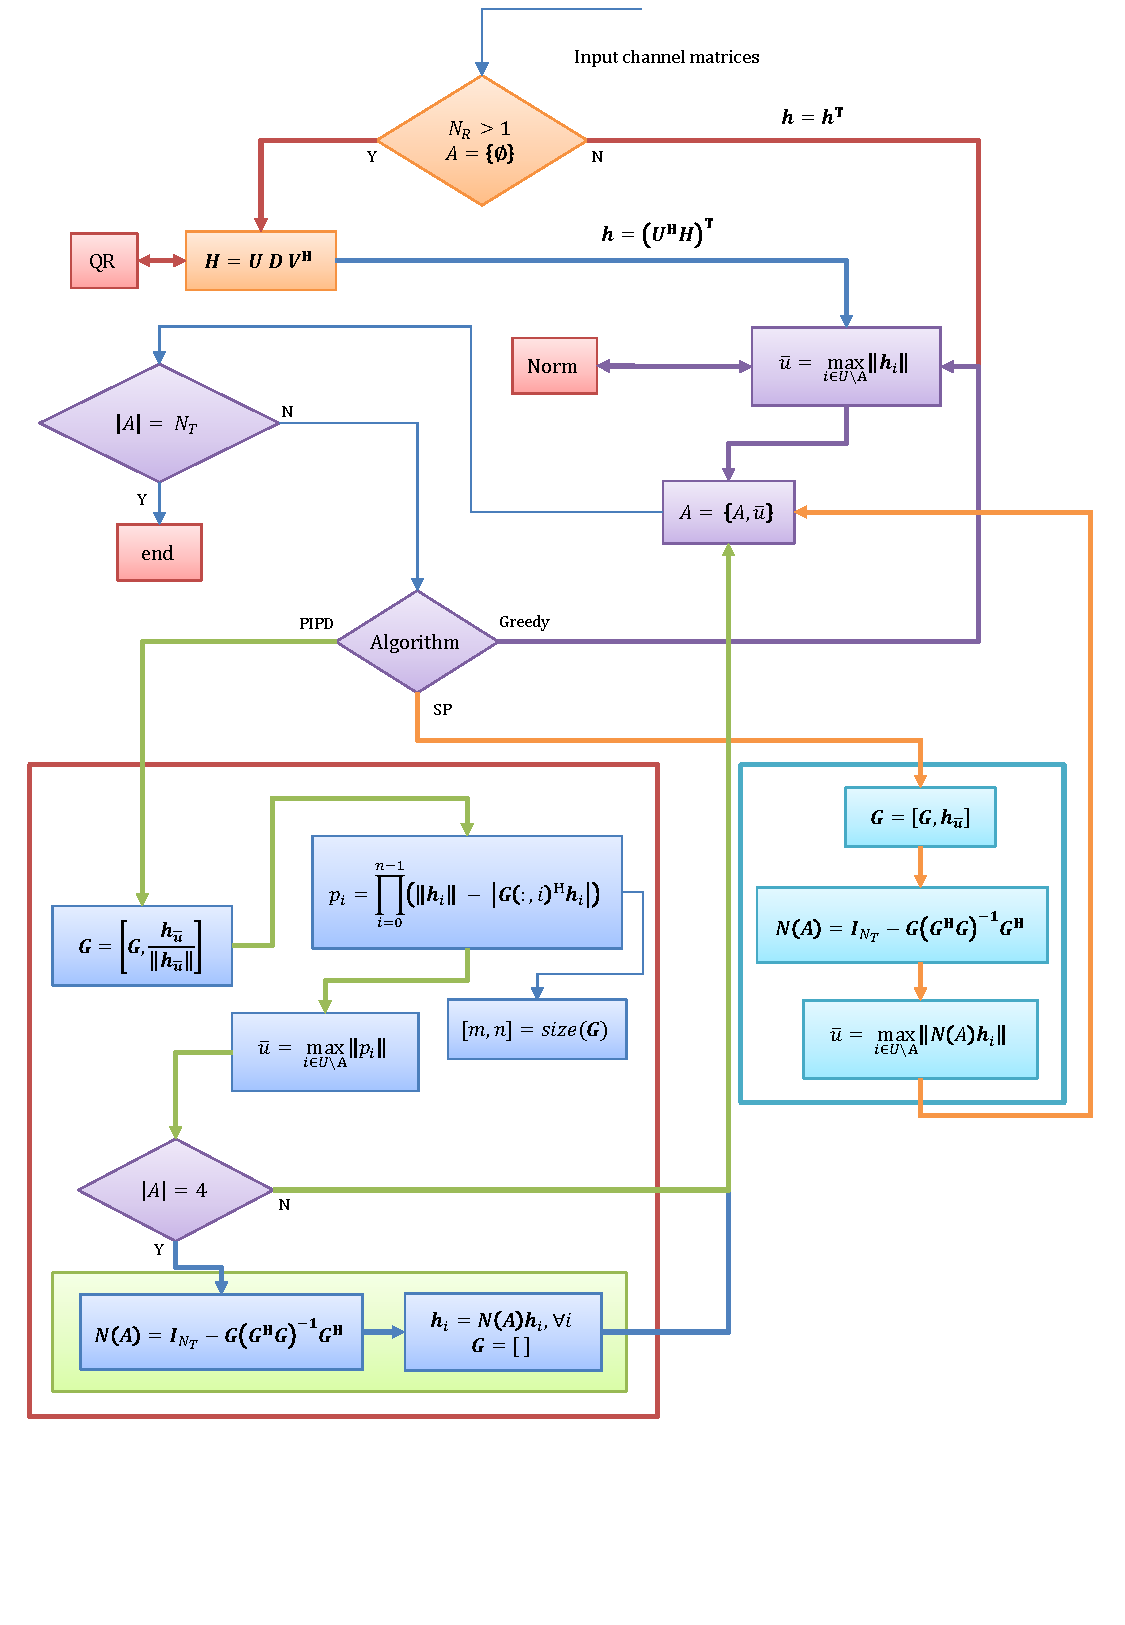
\includegraphics[trim=0in 1.5in 0in 0.75in,width=\columnwidth, angle=0]{Algorithm_Model}
	\caption{Scheduler algorithm flow.}
	\label{kuva:scheduler_block_diag}
	\vspace{-0.1in}
\end{figure}

\section{Scheduling Algorithms}
\label{sec:sched_discussions}
The selection of a subset of users \eqn{\mc{A}} from the set \eqn{\mc{U}} for a sum rate maximization objective requires an exhaustive search, and therefore the complexity is of the order of \eqn{O((K \times N_R)^{N_T})}. In order to reduce the complexity involved in the selection procedure, we find a subset of user channel vectors that are as linearly independent as possible to reduce the inter-stream interference caused by the spatial multiplexing. Fig. \ref{kuva:scheduler_block_diag} shows the outline of the scheduling algorithms discussed in this section. Due to the simplicity of the greedy/norm based search, we omit the discussion on the greedy scheduling algorithm. We assume simple linear precoder design based on zero-forcing (ZF) algorithm on the stacked channel vectors of the chosen users by the scheduling algorithm.

\subsection{Successive Projections (SP)}
The SP scheduling algorithm selects the users in an iterative manner by finding the user channel vectors that are linearly uncorrelated with the already chosen channel vectors. The compatibility is evaluated by projecting the channel vector onto the null space formed by stacking the existing channel vectors of the chosen users from the earlier iterations \cite{sus2006zfbf,antti_user_selection}. Initially, a user with higher channel gain from the set \me{\mc{U}} is selected for the transmission set \me{\mc{A}}. Then, the remaining users are selected from \eqn{\mathcal{U} \backslash \mathcal{A}} by projecting the equivalent channel vectors \me{\mvec{h}{\hat{k}} =\mvec{U}{k}(i)^\herm \mvec{H}{k}} onto the null space of the user channel vectors in \eqn{\mathcal{A}} as
\begin{subeqnarray}
	\mbf{G} &=& \left [ \mvec{h}{\mathcal{A}(1)}^\tran,\dotsc,\mvec{h}{\mathcal{A}(|\mathcal{A}|)}^\tran \right ] \slabel{eqn-1.0} \\
	\mbf{N}(\mathcal{A}) &=& \mbf{I}_{N_T} - \mbf{G} \left (\mbf{G}^\herm \mbf{G} \right )^{-1} \mbf{G}^\herm \slabel{eqn-1.1}
\end{subeqnarray}
where \textbf{N} denotes the null space matrix and $\mbf{I}_{N_T}$ is the identity matrix of size $N_T$. The metric for the selection is given by
\begin{subeqnarray}
	m_i &=& \| \mbf{N}(\mathcal{A}) \, \mvec{h}{i}^\tran \|, \; \forall \, i \, \in \mathcal{U} \backslash \mathcal{A} \label{eqn-1.2}\\
	\bar{u} &=& \underset{i}{\arg \max} \; m_i, \quad \mathcal{A} = \mathcal{A} \cup \set{\bar{u}}.
\end{subeqnarray}
The above metric is evaluated for all users at each iteration to identify a user until the condition $|\mc{A}| = N_T$ is satisfied. Even though selecting \me{N_T} users is not optimal in the lower \ac{SNR} regime, the precoders can be recalculated by retaining the channel vectors with non-zero power. To reduce the complexity, we can ignore the square root involved in the channel norm evaluation that is required for the user searching.

\subsection{Product of Independent Projections (PIPD)}
The PIPD algorithm requires minimal computational complexity compared to the SP scheduling scheme as discussed in \cite{venkatraman2014low}. The complexity involved in selecting the first user remains the same, since the user with the highest channel norm is considered for the set \eqn{\mc{A}} in both schemes. The complexity involved in selecting the remaining users for set \me{\mc{A}} is significantly reduced in the PIPD scheduling scheme by virtue of using the product of independent vector projection displacements metric. A detailed description of the algorithm can be found in \cite{venkatraman2014low}. However, for a system configuration of \me{N_T = 8} antennas, the performance of the PIPD scheme is significantly inferior to that of the SP scheduling algorithm. To overcome this problem, we modified the PIPD algorithm as highlighted in Fig. \ref{kuva:scheduler_block_diag} by projecting user channel vectors onto the null space of the existing user channels when \me{|\mc{A}| = 4}. Once the channel vectors are projected onto the null space formed by the existing user set \eqn{\mc{A}}, the algorithm proceeds by finding the remaining users for the active user set \eqn{\mc{A}}. It can also be restarted to search the remaining \eqn{N_T - 4} users for the transmission set \eqn{\mc{A}}, since current \eqn{\mbf{G}} matrix provides zero valued vector. At this point, the next user selection is simply based on the max norm of the already projected channel vectors and then proceeds as earlier. It reduces the overall complexity involved in the search algorithm by limiting the matrix inversion only to the maximum of \eqn{4 \times 4} matrix.

Fig. \ref{kuva:scheduler_block_diag} illustrates the operations involved in the metric calculations for greedy, SP and PIPD scheduling schemes. The blocks mentioned separately for the PIPD and the SP schemes are executed based on the selected algorithm. The greedy algorithm requires only the norm calculation of the virtual channel vectors with which the sorting operation can be used to find the leading $N_T$ users for set $\mathcal{A}$. In case of the SP selection scheme, the users are identified by projecting the corresponding channel vectors onto the null space of the existing users, channel vectors and selecting the one with the maximum projection gain. In order to evaluate the null space, a matrix inversion is needed, which incurs significant amount of processing power in comparison to the vector multiplications involved in the PIPD algorithm in Fig. \ref{kuva:scheduler_block_diag}.

\section{Performance of MU-MIMO Scheduling}
\label{sec:perf_scheduling}
\subsection{Scheduling Resolution}
The user selection is performed over each scheduling block (SB). The number of SBs in the system determines the overall achievable throughput. For instance, if the SB resolution is equal to the physical resource block (PRB), the scheduling complexity increases linearly with the number of SBs and the throughput performance depends on the number of users in the system. Thus, if the number of users is large, the performance will improve by utilizing the multi-user diversity with the help of a proper scheduling scheme. However, if the users are few in number, the performance degradation is significant due to the smaller coding length and lack of channel variations over the smaller SB to extract the channel diversity in the form of coding gain. In case of a larger SB size with grouped PRBs, the scheduling complexity will be reduced significantly, but the network throughput will also reduce noticeably unless the channel fading over frequency domain is flat or nearly flat. In this case, the users with the transmission in such scheduling will attain higher throughput due to the longer coding length which needs to be quantified only by the system level study.
\begin{figure}
	\centering
	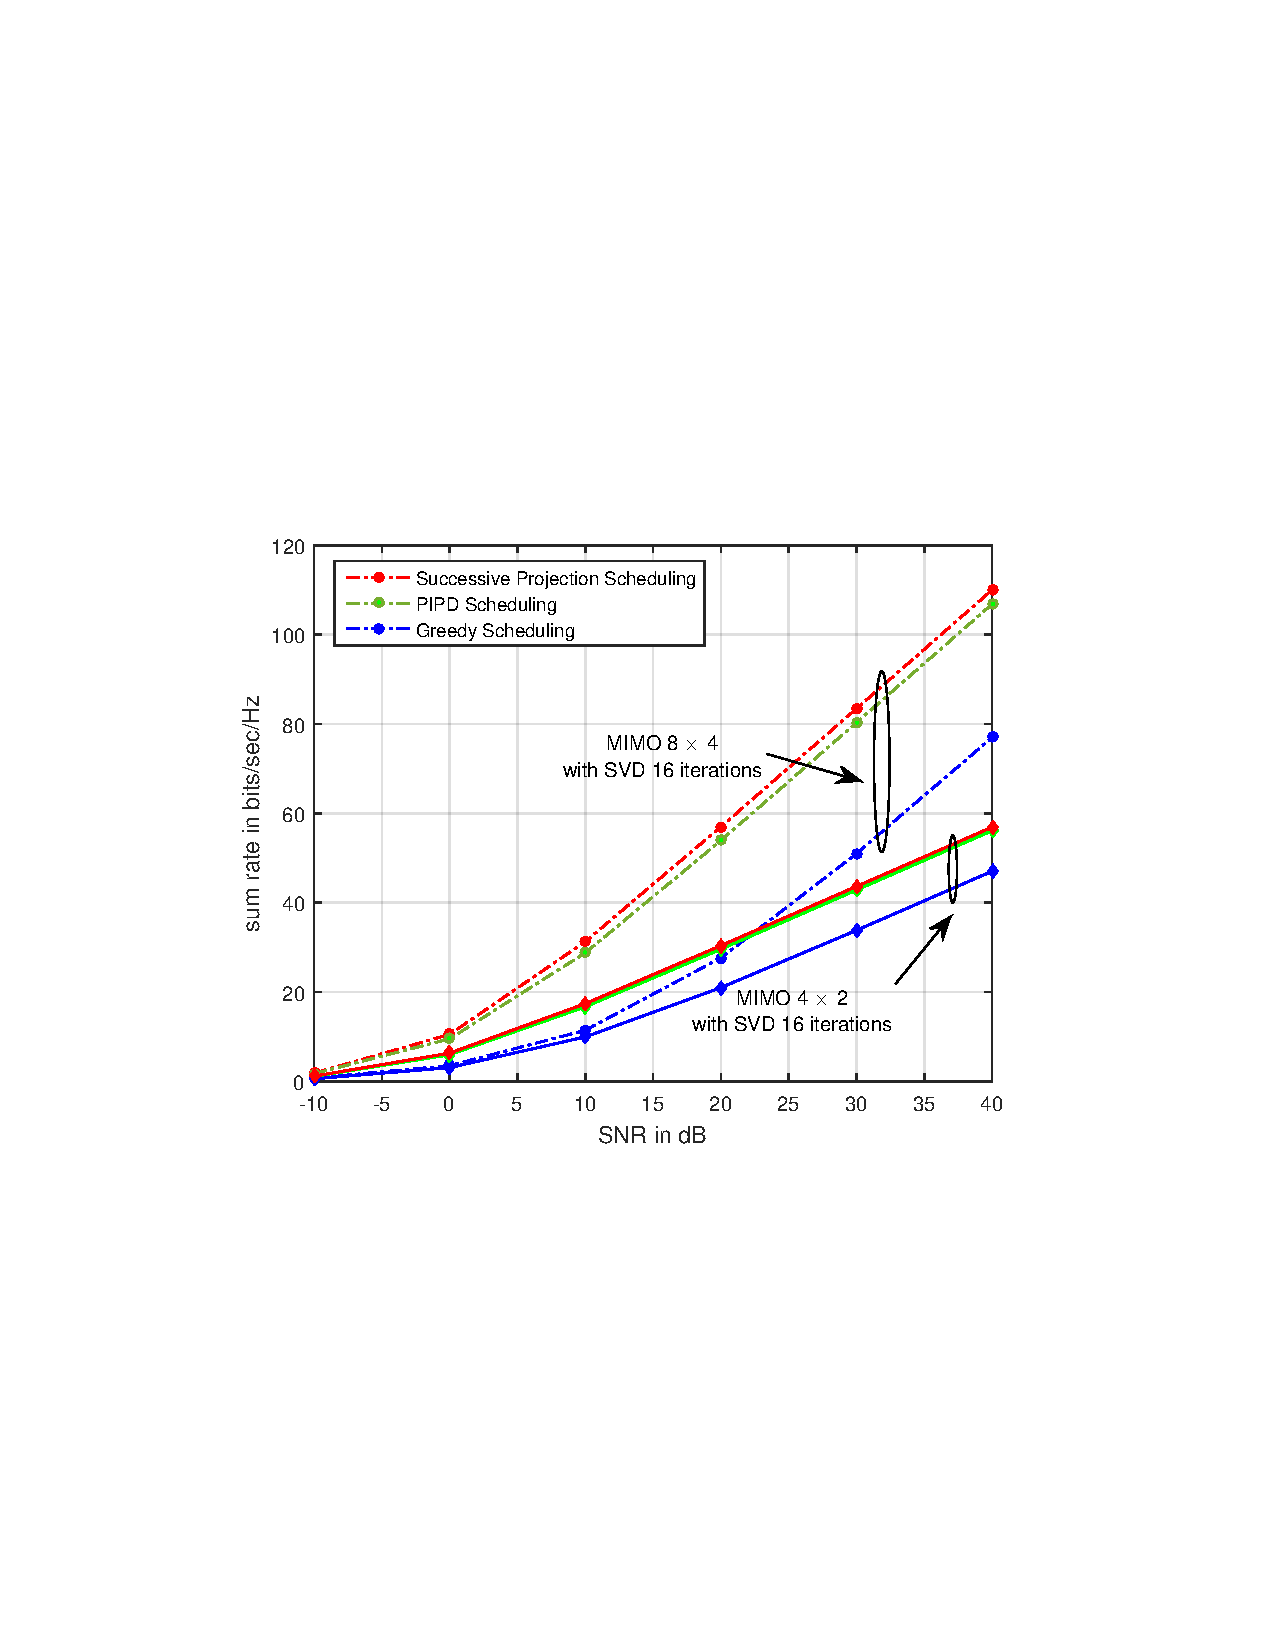
\includegraphics[trim=1.5in 3.5in 1.5in 3.5in,width=\columnwidth]{sra_100}
	%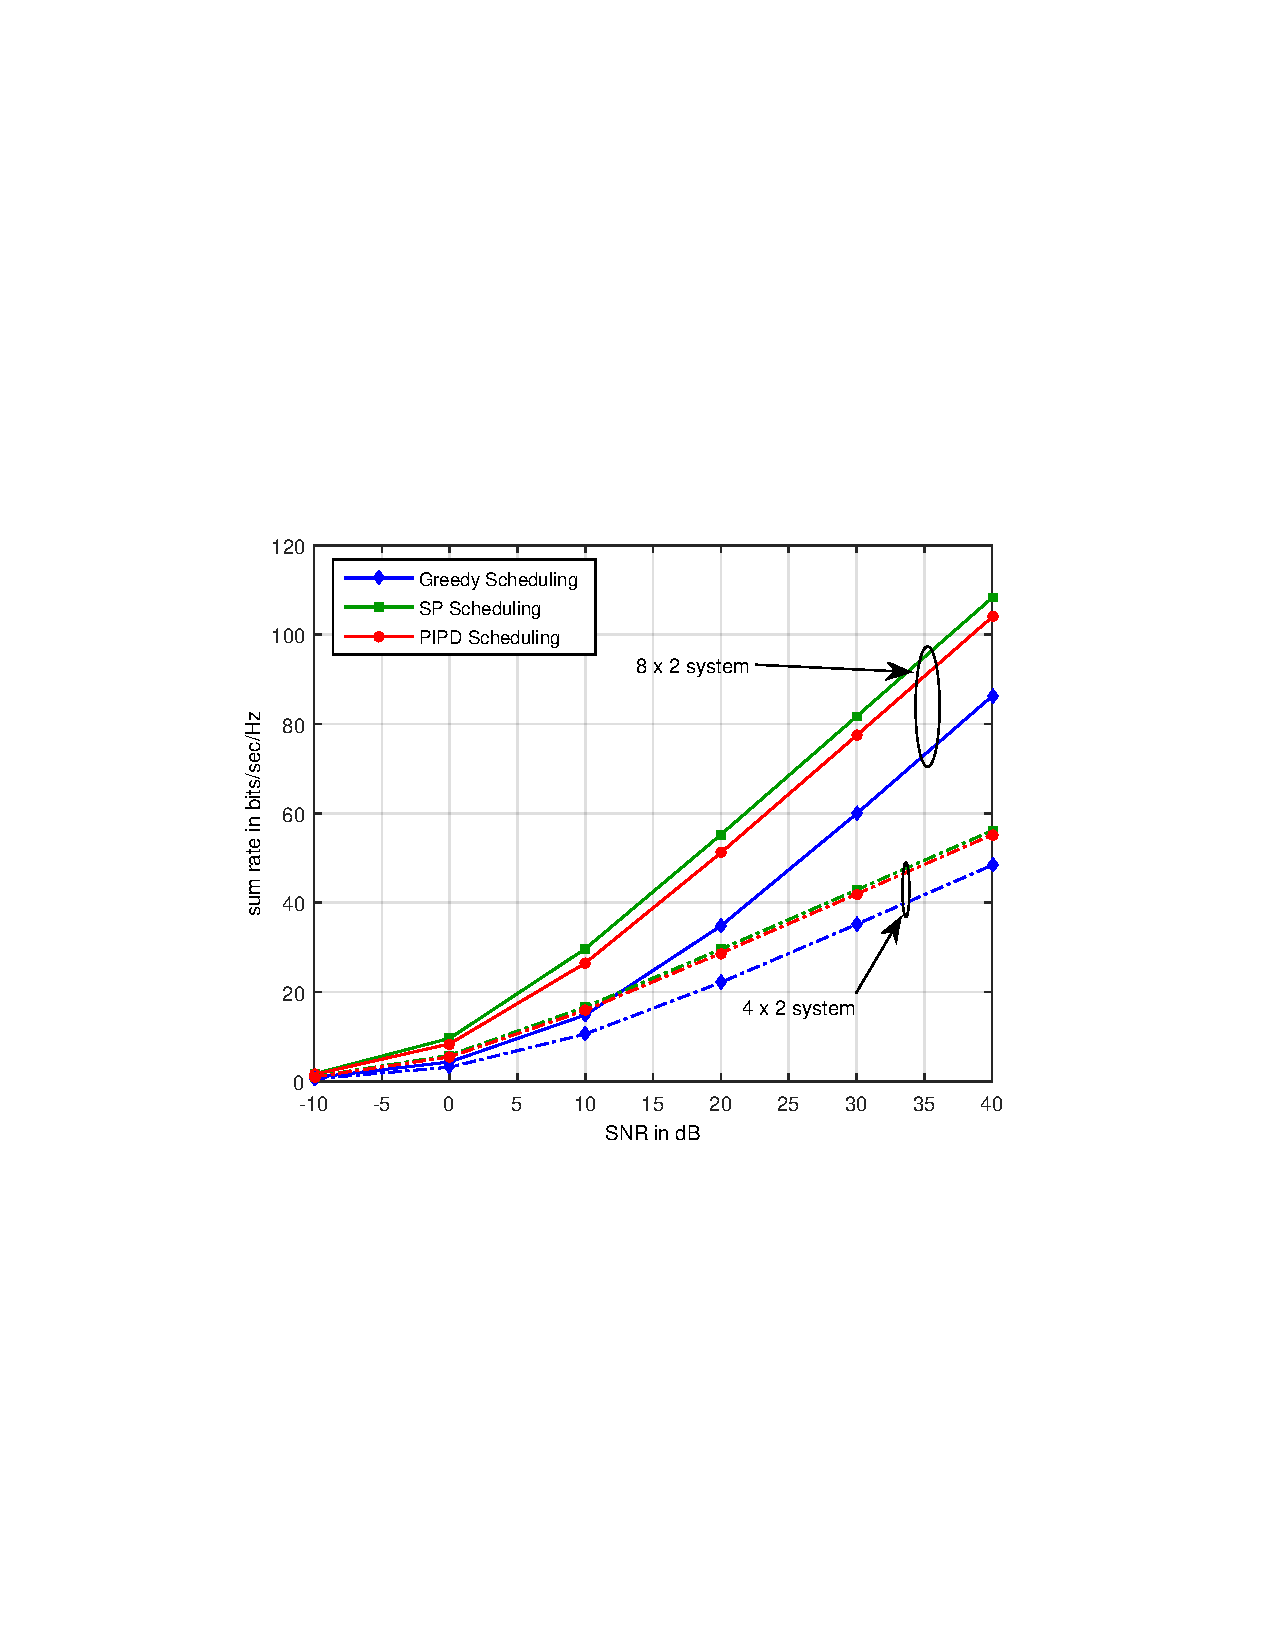
\includegraphics[width=\columnwidth]{sra_50_users}
	\caption{Comparison of scheduler algorithms for $K = 100$ users.}
	\label{kuva:performance_plot}
	\vspace{-0.15in}
\end{figure}

\subsection{Scheduling Performance}
Fig. \ref{kuva:performance_plot} compares the sum rate performance of three different scheduling schemes with $\textrm{N}_T = 4,8$ and $K = 100$ users. The sum rate of the PIPD scheme performs significantly close to the SP scheme. Fig. \ref{kuva:performance_plot} also shows a larger gap (approximately 10 bit/sec/Hz) between Norm/Greedy scheme which selects users based on the channel norm only and PIPD scheduling scheme for a \eqn{4 \times 2} configuration. Note that the performance of the scheduling algorithms improves marginally by adding additional receive antennas, due to the channel hardening by the multi-user diversity. Increasing \me{N_T} antennas in the system, improves the achievable sum rate of the system by multiplexing more number of users over the spatial dimension, which is evident from Fig. \ref{kuva:performance_plot}.

\section{Implementation Results}
\label{sec:implementation}
In this section, we discuss the fixed point implementation of various scheduling algorithms discussed in the Section \ref{sec:sched_discussions} on TI's Keystone-II platform. For the current implementation work, we considered only single SB scenario and utilize the available \eqn{N_C=8} cores in the evaluation platform. 

\subsection{SVD Implementation}
The SVD is performed by repeated QR factorization to obtain the left and the right singular vectors of the channel matrices. The complex QR decomposition is performed using the Householder transformations \cite{aft}. We perform \eqn{16} QR factorization for each SVD processing to limit the off diagonal values of the \eqn{\mvec{D}{k}} matrix \eqn{\leq 1e^{-4}}. The SVD requires significant computational complexity and time, and therefore, it is ideal to perform in parallel over multiple cores. Since the matrix size is typically limited by the number of transmit and the receive antennas, parallelizing each SVD operation is not an efficient approach due to the overhead involved in setting up the resources for sharing and synchronization. In the current approach, each TI C66x core shares \eqn{\lfloor \frac{K}{N_C} \rfloor} of the available SVD operations to perform in parallel.
	
The channel matrices are stored in \ac{MSMCSRAM}, and therefore accessible from all cores in the \ac{SoC}. In this work, only Core(0) is used to perform scheduling and all other cores are utilized for the SVD processing. Due to the availability of the shared memory \ac{MSMCSRAM} region, we can synchronize the cores effectively by using shared memory and \ac{IPC} interrupts available through \ac{CIC} instead of using OpenMP framework \cite{openmp,ipc,cic}. Since each core is running separate SYS-BIOS operating system, the shared memory region addressing will be different for each cores. In order to overcome the memory aliasing, we fix the channel buffer to a fixed physical address using the compiler directive \textit{location} so as to be coherent with the channel buffer location. The channels are randomly generated and stored in the shared memory region. An interrupt is given to all the cores to notify the availability of the updated channel state information and to start processing for the SVD operation in parallel.

At this point, each core determines the starting offset in the buffer based on the number of cores sharing the computation and the current core number. If the total number of channel matrices is not an exact multiple of the number of cores, then the first \eqn{\textrm{mod} (K,N_C)} processors perform one additional SVD processing to share the overall load. In the current scenario, Core(0) performs the scheduling of users. Therefore, after completing the SVD of the channel matrices, instead of waiting for other cores to complete the SVD job, Core(0) can proceed with the scheduling algorithm after invalidating the relevant buffers without affecting the overall selection procedure as shown in Fig. \ref{sched_cores}. Meanwhile, other cores will complete and write back all the virtual channel matrices to the shared \ac{MSMCSRAM} from the cache before switching to the idle task. We notify the availability of the channels using \ac{CIC} interrupt to all cores as shown in Fig. \ref{sched_cores}.
\begin{figure}
	\centering
	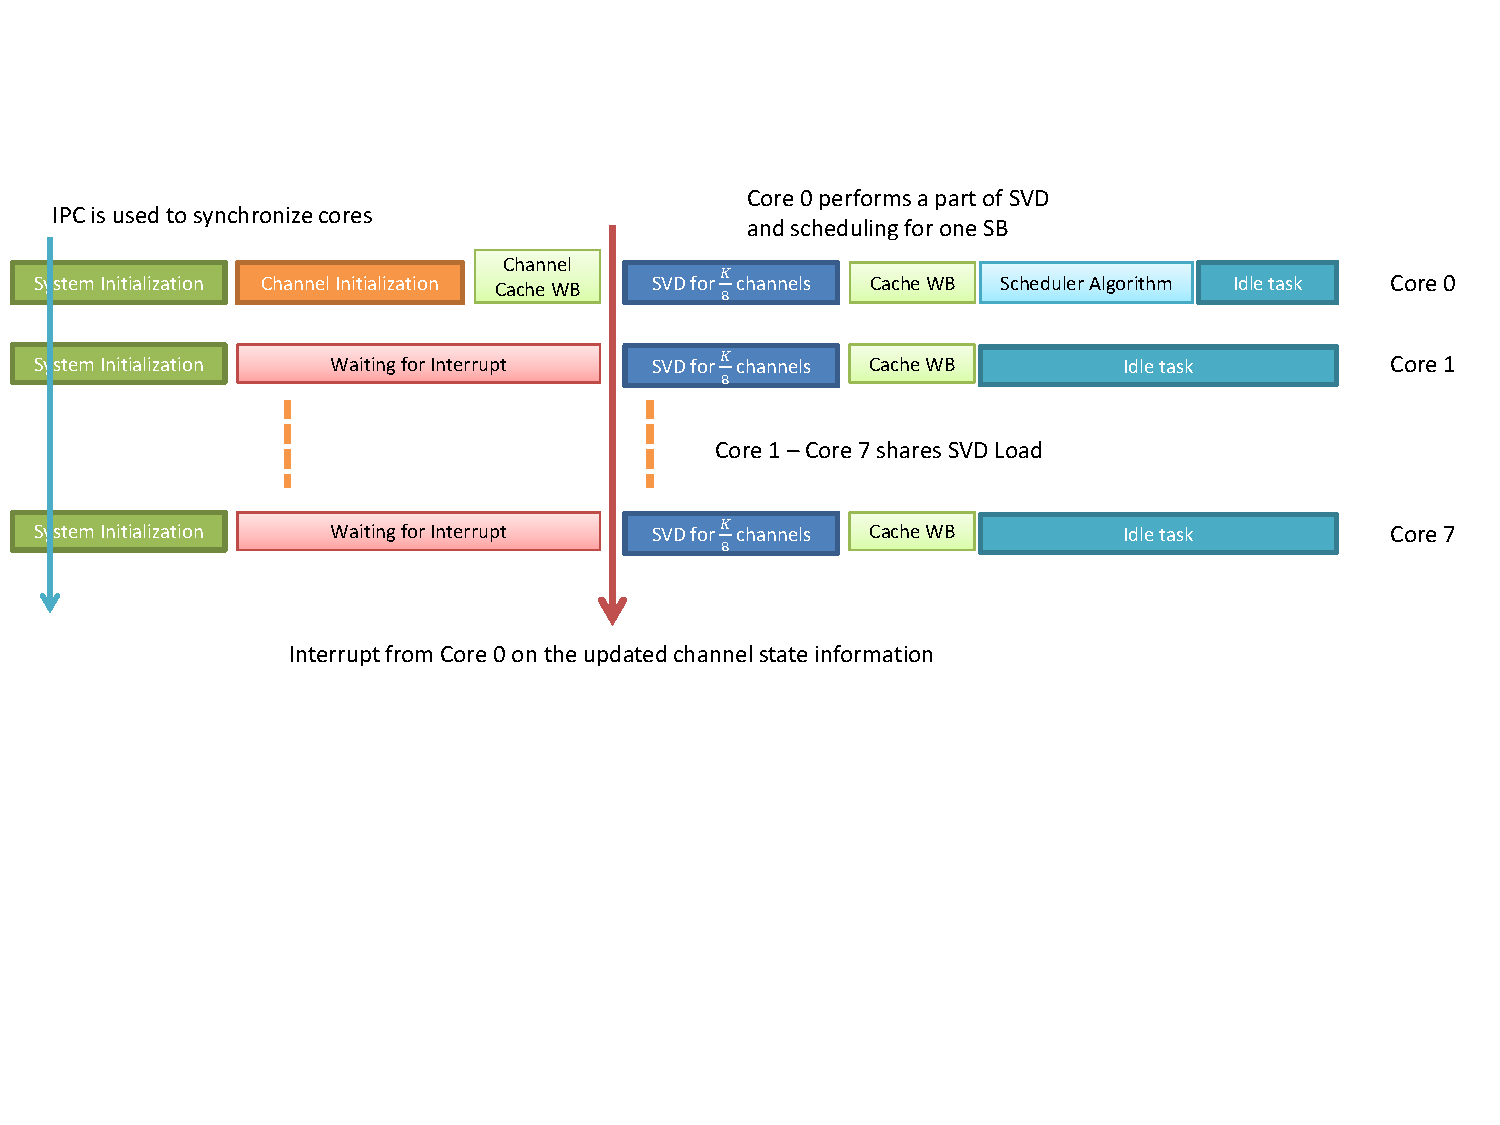
\includegraphics[trim=0in 3.25in 0in 1.5in,width=\columnwidth]{overall_scheduling}
	%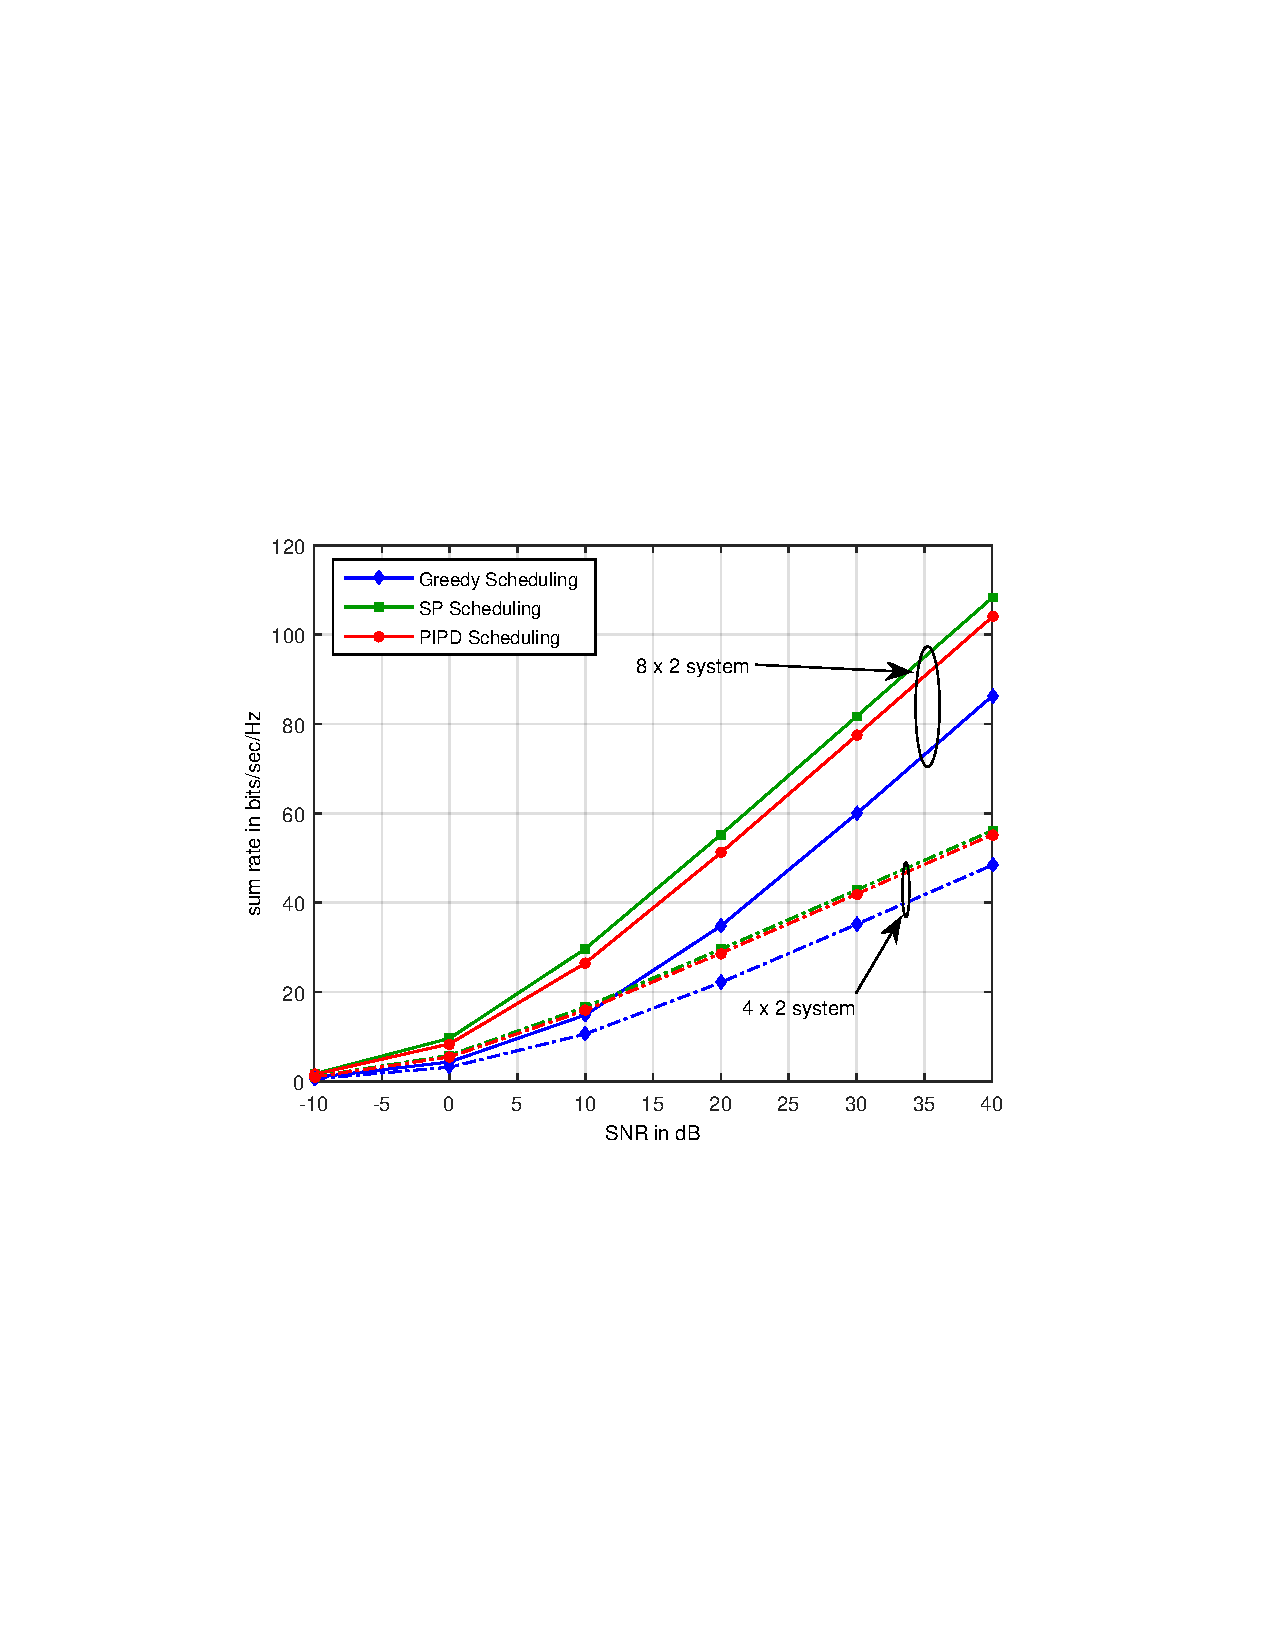
\includegraphics[width=\columnwidth]{sra_50_users}
	\caption{Task scheduling over \eqn{N_C = 8} cores.}
	\label{sched_cores}
	\vspace{-0.15in}
\end{figure}

\subsection{Scheduler Implementation on C66x}
The scheduling algorithms and the overall control is performed by Core(0). Since we analyze only single SB in the current work, we utilize only C66x Core(0) to perform user scheduling. In order to reduce the computational latency, we implement all the algorithms and the SVD computation in fixed point format. The complex baseband channel is represented in a packed real and imaginary format with \eqn{16} bit representation by allocating \eqn{15} bits for the fractional part and one bit to represent the sign. Since the output of the SVD is also used in the precoder design, Core(0) writes back the virtual channel buffer before proceeding with the user scheduling. The complex operations involved in the scheduling algorithms are null space evaluation and the matrix-by-vector multiplications. In order to evaluate the actual timing of the scheduling algorithm, we invalidate the cache of Core(0) before the scheduling algorithm. The complexities of various schemes are tabulated in Table \ref{table:compexity_comparison}. Note that the overall complexity involved in the scheduler implementation can be reduced by limiting the stream search to the dominant streams only, since the singular values are sorted in the descending order. Due to the available multi-user diversity, limiting the stream search has marginal impact on the sum rate performance. 

Table \ref{table:compexity_comparison} compares the complexity of various algorithms using the time as the metric for \eqn{K = 100} users. The legend \me{\lambda} in Table \ref{table:compexity_comparison} denotes the number of streams included in the scheduler algorithm search. It can take the maximum value of \me{\kappa}, which is the rank of the channel. As seen from Table \ref{table:compexity_comparison}, significant amount of time is spent on the SVD computations. From Table \ref{table:compexity_comparison}, we can see that the total time taken by performing SVD in parallel is significantly less when compared with the single core performance. Note that the multi-core performance is not equal to the single core timing if it is multiplied by the number cores. It is due to the overhead involved in the cache coherency and also due to the unequal sharing of the load of $K = 100$ channel matrices.
\begin{table} \caption{Scheduling Complexity for $K = 100$ users ($\mathrm{msec}$) with C66x operating at \eqn{1.2}GHz} \begin{center} \begin{tabular}{c c c c c c c}
			$N_T \times N_R $ & $\lambda$ & SVD \eqn{(1)} & SVD \eqn{(8)} & Greedy   & SP          & PIPD \\ 
			\hline \\
			$8 \times 4$ & 4 & 22.68 & 2.90 & 0.075 & 0.524 & 0.469 \\ 
			$8 \times 4$ & 2 & 22.68 & 2.90 & 0.064 & 0.325 & 0.268 \\
			$8 \times 2$ & 2 & 6.055 & 0.79 & 0.063 & 0.325 & 0.266 \\
			$8 \times 2$ & 1 & 6.055 & 0.79 & 0.058 & 0.226 & 0.166 \\
			\hline \\
			$4 \times 4$ & 4 & 15.81 & 2.07 & 0.045 & 0.168 & 0.167 \\ 
			$4 \times 4$ & 2 & 15.81 & 2.07 & 0.034 & 0.102 & 0.098 \\
			$4 \times 2$ & 2 & 4.844 & 0.64 & 0.034 & 0.102 & 0.097 \\
			$4 \times 2$ & 1 & 4.844 & 0.64 & 0.029 & 0.069 & 0.063 \\
			\hline \vspace{-0.3in}
		\end{tabular} \label{table:compexity_comparison}\end{center}
\end{table}

As far as the scheduler complexity is concerned, we can see that all the scheduling algorithms can meet the LTE-A timing requirements for the user scheduling, which happens at the sub-frame interval of \eqn{1} msec. The complexity of the SP and the PIPD algorithm is attributed to the null space matrix evaluation. Note that the square root is not performed for the norm calculation in the SP and in the greedy scheduling scheme, which provides additional margin. The complexity of the SP algorithm is due to both null space evaluation and the matrix-by-vector multiplication. The SVD operation can be performed over the radio frame of \eqn{10} msec. duration, which can be justified by the nomadic user assumption with the slowly changing channel fading.

The computational figures provided in Table \ref{table:compexity_comparison} for the SVD scales linearly with each additional user in the system and it increases with the number of users $K$ with each additional SB. The complexity of the scheduling algorithms scales linearly with the additional number of SBs while with the number of users, it is sublinear. Table \ref{table:compexity_comparison} also provides information about the scalability of the system with the number of SBs that can be supported by the \ac{SoC} implementation without compromising the real-time constraints. For example, assuming the channel is coherent for \eqn{10} ms, we can support \eqn{8} SBs with \eqn{8 \times 2} MIMO configuration by performing all SVDs related to $K = 100$ users in \eqn{6.055} msec and any scheduling algorithm at $1$ msec interval. In this approach, each SB is served by each core dedicatedly without any real-time performance glitch. Note that if we reduce the number of QR iterations in each SVD, we can support $10$ SBs with slight degradation in the performance.

\acresetall \acused{MIMO}
\section{Conclusions and Future Work}
\label{sec:conclusion}
We studied the computational complexity of different state-of-the-art MU-MIMO scheduling algorithms. We showed that the complexity is mainly attributed to the SVD decomposition of the channel matrices and the matrix multiplications involved in the metric calculations. We have demonstrated the performance of three different scheduling algorithms on TI TCI6636K2H evaluation platform by sharing the SVD operations over multiple C66x DSP cores. In future, we analyze the performance of the scheduling algorithms on four ARM cores by performing only SVDs on the available C66x DSP cores.

\section*{Acknowledgment}
This research was done in BaSE (Baseband and System Technologies for Wireless Evolution) project supported by the Finnish Funding Agency for Innovation (Tekes), Nokia, Broadcom, Xilinx and Elektrobit.

\bibliographystyle{./../../IEEE/IEEEtran}
\bibliography{./../../IEEE/IEEEabrv,./../biblio/bibliography}
%\bibliography{./../biblio/bibliography}

\end{document}
